\documentclass[tikz,border=5pt]{standalone}
\usetikzlibrary{spath3,intersections}
\begin{document}
    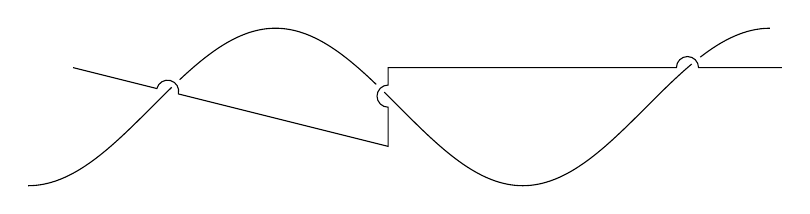
\begin{tikzpicture}
        \coordinate (a) at (-1,0.5);
        \coordinate (b) at (8,0.5);
        \coordinate (c) at (3,-0.5); 
        \path[spath/save=sine]
            (-1.57,-1)
            cos ++(1.57,1)
            sin ++(1.57,1)
            cos ++(1.57,-1)
            sin ++(1.57,-1)
            cos ++(1.57,1)
            sin ++(1.57,1);
        \path[spath/save=over] (a) -- (c) |- (b);
        \path[spath/save=arc] (0,0) arc[radius=1cm, start angle=180, delta    angle=-180];

        \tikzset{
            spath/split at intersections with={over}{sine},
            spath/insert gaps after components={over}{8pt}, 
            spath/join components upright with={over}{arc}, 
            spath/split at intersections with={sine}{over}, 
            spath/insert gaps after components={sine}{4pt},
        }

        \draw[spath/use=sine]; 
        \draw[spath/use=over]; 
    \end{tikzpicture}

    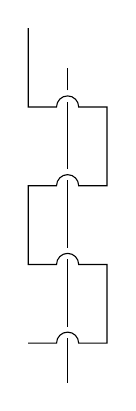
\begin{tikzpicture}%
        \tikzset{%
            bridging path/.initial=arc,
            bridging span/.initial=8pt, 
            bridging gap/.initial=4pt, 
            bridge/.style 2 args={%
                spath/split at intersections with={#1}{#2}, 
                spath/insert gaps after components={#1}{\pgfkeysvalueof{/tikz/bridging span}}, 
                spath/join components upright  with={#1}{\pgfkeysvalueof{/tikz/bridging path}}, 
                spath/split at intersections with={#2}{#1}, 
                spath/insert gaps after components={#2}{\pgfkeysvalueof{/tikz/bridging gap}},
            }%
        }%
        \tikz[overlay] { \path[spath/save global=arc] (0,0) arc[radius=1cm,start angle=180, delta angle=-180]; }%    
        \path[spath/save=over] (0,0) -| ++(1,1) -| ++(-1,1) -| ++(1,1) -| ++(-1,1);
        \path[spath/save=under] (.5,-.5) -- ++(0,4);
        \tikzset{bridge={over}{under}} 
        \draw[spath/use=over]; 
        \draw[spath/use=under]; 
    \end{tikzpicture}
\end{document}
